
%(BEGIN_QUESTION)
% Copyright 2011, Tony R. Kuphaldt, released under the Creative Commons Attribution License (v 1.0)
% This means you may do almost anything with this work of mine, so long as you give me proper credit

Suppose a radio antenna receives 0.52 watts of power from the end of a twin-lead cable connected to an RF transmitter.  The cable is 30 feet long, and exhibits a power loss of $-0.041$ dB/foot.  Calculate the output power of the transmitter, in both units of watts and units of dBm.

\vskip 10pt

$P_{xmtr}$ = \underbar{\hskip 50pt} watts

\vskip 10pt

$P_{xmtr}$ = \underbar{\hskip 50pt} dBm

\vskip 10pt

Finally, determine if your calculations for transmitter power would be any different if you knew the antenna had a gain of +6.8 dBi.

\vskip 20pt \vbox{\hrule \hbox{\strut \vrule{} {\bf Suggestions for Socratic discussion} \vrule} \hrule}

\begin{itemize}
\item{} A technique highly recommended for word-problems is to {\it sketch a picture} of the problem and label elements of that picture with the given information.  Do this, and compare your sketch with those of your classmates.  How, specifically, does this aid your problem-solving?
\item{} If the operating frequency of this radio system were increased, would cable loss increase, decrease, or remain the same as before?
\item{} If the operating frequency of this radio system were increased, would the antenna need to be lengthened, shortened, or would the same antenna work just as well as before?
\end{itemize}


\underbar{file i02533}
%(END_QUESTION)





%(BEGIN_ANSWER)

\noindent
{\bf Partial answer:}

\vskip 10pt

$P_{xmtr}$ = \underbar{\bf 0.6902} watts


%(END_ANSWER)





%(BEGIN_NOTES)

Sketching a picture of the problem is strongly recommended as a problem-solving technique:

$$\includegraphics[width=15.5cm]{i02533x01.eps}$$

A 30-foot-long cable having a loss of $-0.041$ dB per foot will exhibit a total loss of $-1.23$ dB along its entire length.  This means the power received at the antenna will be less than the transmitter's output power by the following ratio:

$$10^{-1.23 \over 10} = 0.7534$$

Thus, is the antenna is receiving 0.52 watts from the cable, the cable must be receiving $1 \over 0.7534$ times as much power from the transmitter, or 0.6902 watts.  This transmitter power of 0.6902 watts equates to {\bf 28.39 dBm}.

\vskip 10pt

Antenna gain has no bearing whatsoever in this case, because that only affects how much of the 0.52 watt power gets radiated into space in a particular direction, not how much power is lost over the length of the cable.

%INDEX% Electronics review: decibel power calculations

%(END_NOTES)


